\section{Журнал выполнения}
\begin{enumerate}
    \item Где хранить частоты. Отдельный файл рядом с индексом пришлось бы читать параллельно со списками; поэтому частоты --- прямо в записях списков (пары docID, tf), а длина вектора документа --- в его записи прямого индекса. Формат BIDX это допускал: размер записи документа берётся из заголовка, а новые возможности включаются флагами. Без ключа \texttt{-t} индекс тот же, что раньше; автотесты ЛР4, ЛР7, ЛР8 и ЛР11 после изменений пройдены.
    \item Один тест ЛР11 проверял, что индекс с \enquote{неизвестным} флагом 4 не открывается, --- теперь это флаг частот. В тесте неизвестным стал флаг 8.
    \item Память индексации выросла с 2,1 до 4,0~ГиБ: на каждую запись списка в памяти добавилась частота (4 байта). Хватило бы 1--2 байт с насыщением или хранения списков в памяти сразу кодами VByte.
    \item Первые прогоны показали, что лучше всего ранжируются короткие документы: посты Reddit и вопросы Travel SE, а длинные статьи, целиком посвящённые предмету запроса, опускаются (примеры ниже). Это свойство косинусной нормировки lnc: вес слова делится на длину вектора всего документа. Схема оставлена как в задании и лекции; способы исправления --- в выводах.
    \item В булевом режиме оценки накапливаются по полным спискам всех слов запроса, а не только по найденным документам. Это просто и одинаково с нечётким режимом, но медленно для частых слов (\texttt{to}, \texttt{the} --- почти миллион записей).
    \item Разметка. Посты Reddit в корпусе --- только текст вопроса, без комментариев, поэтому пост по теме оценщики оценивали не выше 1. Двоек всего 16 из 282 (175 нулей, 91 единица): статьи-обзоры и ответы Travel SE. Оценщики отмечали спорные случаи (например, путеводители по странам с советами для женщин для запроса 8 --- 1, при более мягком подходе 2).
    \item Веб-сервис ЛР8 показывает оценку TF-IDF под каждым результатом; заодно исправлена подпись главной страницы (там ещё было \enquote{30\,000 статей}).
\end{enumerate}

\section{План тестирования}
Юнит-тесты на C++ (\texttt{tests/test\_rank.cpp}) на каркасе \texttt{lab3/tests/unittest.h}; запуск --- \texttt{make test}. Эталоны считаются независимо от проверяемого кода: косинус lnc.ltc по словарям частот на контейнерах STL, свой разбор файла индекса по описанию формата.

\begin{center}
\small
\begin{tabular}{|c|p{0.3\textwidth}|p{0.58\textwidth}|}
\hline
\textnumero & Тест & Что проверяется \\
\hline
1 & Веса lnc.ltc & idf = $\log_{10}(N/\mathit{df})$, вес tf = $1 + \log_{10} \mathit{tf}$; пример лекции \enquote{best car insurance} даёт оценку 0,80. \\
\hline
2 & Нечёткий или булев & Запрос только из слов --- нечёткий, с любым из \texttt{\& | ! ( )} --- булев. \\
\hline
3 & Формат индекса с частотами & Свой разбор файла: флаги 4 и 6, запись документа 16 байт, длины векторов документов, пары (docID, tf) без сжатия (по 8 байт) и со сжатием; распаковка отвергает $\mathit{tf} = 0$. \\
\hline
4 & Булев поиск по индексу с частотами & \texttt{read\_list} и поиск ЛР8 дают одно и то же по индексам без частот и с ними (без сжатия и со сжатием). \\
\hline
5 & Ранжирование на маленьком корпусе & Нечёткий запрос находит документы хотя бы с одним словом, документ с обоими словами выше, короткий выше длинного, оценки равны эталонным; булев \texttt{rose \&\& flower} строгий; НЕ отсекает, но не влияет на оценку; редкое слово весит больше; запрос из одних НЕ --- оценки 0. \\
\hline
6 & 300 случайных запросов & Корпус из 2000 документов, нечёткие и булевы запросы (И, ИЛИ, НЕ, скобки): множество найденных, оценки (с точностью $10^{-9}$) и порядок совпадают с эталоном; индексы без сжатия и со сжатием дают одно и то же. \\
\hline
7 & Сортировка выдачи & Своя сортировка слиянием 100\,000 оценок с повторами совпадает с \texttt{std::stable\_sort}: по убыванию оценки, при равенстве по docID. \\
\hline
8 & Флаги 1 + 2 + 4 & Стемминг, сжатие и частоты вместе (\texttt{flags} = 7): \texttt{museums} $\to$ \texttt{museum}, ранжирование работает. \\
\hline
9 & Утилиты & \texttt{indexer -t}, \texttt{search} (нечёткий и булев запрос, пятый столбец --- оценка, режим \texttt{-p} веб-сервиса), \texttt{search} по индексу без частот --- прежний булев поиск, \texttt{lookup}. \\
\hline
\end{tabular}
\end{center}
Кроме юнит-тестов, ранжирование проверено на всём корпусе оценкой качества (ниже) и тестами веб-сервиса и поиска ЛР8 (пройдены).

\section{Результаты}
\subsection{Автотесты}
Пройдены все 9 тестов. Журнал прогона (\texttt{results/tests.log}):

{\scriptsize
\VerbatimInput[breaklines, breakanywhere]{../results/tests.log}
}

\subsection{Индекс с частотами}
\texttt{indexer -c -t} на корпусе в 1\,000\,000 документов: 173~с (без частот --- 148~с, ЛР7), пиковая память 4,0~ГиБ (без частот --- 2,1~ГиБ). Размеры (МиБ):
\begin{center}
\small
\begin{tabular}{|l|r|r|r|}
\hline
Индекс & Таблица документов & Списки документов & Весь файл \\
\hline
ЛР7: без частот, без сжатия & 11,4 & 1\,388,4 & 1\,583,9 \\
\hline
ЛР11: без частот, VByte & 11,4 & 419,2 & 614,8 \\
\hline
ЛР13: частоты, VByte & 15,3 & 766,7 & 966,0 \\
\hline
\end{tabular}

\end{center}
Частоты почти удвоили сжатые списки (419 $\to$ 767~МиБ): разность docID занимает в среднем 1,2 байта, а частота почти всегда меньше 128 --- ещё 1 байт. Но индекс с частотами и сжатием всё равно в 1,6 раза меньше исходного индекса ЛР7 без частот.

\subsection{Скорость}
Время выполнения запроса без вывода, повтор 10 раз, минимум из 3 запусков:
\begin{center}
\small
\begin{tabular}{|p{0.45\textwidth}|r|r|}
\hline
Показатель & Булев (ЛР8) & TF-IDF (ЛР13) \\
\hline
Загрузка индекса, мс & 831 & 510 \\
\hline
24 запроса ЛР8: медиана, мс & 0,67 & 8,24 \\
\hline
24 запроса ЛР8: среднее, мс & 2,58 & 34,36 \\
\hline
24 запроса ЛР8: максимум, мс & 23,9 & 163,2 \\
\hline
\end{tabular}

\end{center}
{\footnotesize
\setlength{\tabcolsep}{4pt}
\begin{center}
\begin{tabular}{|r|p{0.25\textwidth}|r|r|r|r|r|r|}
\hline
\textnumero & Запрос & \multicolumn{2}{c|}{Булев (ЛР8), по docID} & \multicolumn{2}{c|}{TF-IDF, нечёткий} & \multicolumn{2}{c|}{TF-IDF, строгое И} \\
\hline
 &  & найдено & мс & найдено & мс & найдено & мс \\
\hline
1 & \texttt{cheap hostels paris} & 553 & 0,28 & 103\,660 & 10,15 & 553 & 2,90 \\
\hline
2 & \texttt{best time to visit iceland} & 710 & 1,51 & 981\,586 & 107,30 & 710 & 27,23 \\
\hline
3 & \texttt{visa requirements russian citizens} & 373 & 0,27 & 129\,313 & 12,92 & 373 & 3,57 \\
\hline
4 & \texttt{snorkeling coral reefs thailand} & 38 & 0,04 & 40\,322 & 3,47 & 38 & 0,88 \\
\hline
5 & \texttt{moscow aviation institute} & 475 & 0,14 & 86\,504 & 8,10 & 475 & 1,83 \\
\hline
6 & \texttt{lviv old town} & 350 & 0,26 & 361\,503 & 35,62 & 350 & 7,06 \\
\hline
7 & \texttt{train london edinburgh} & 2\,129 & 0,29 & 182\,941 & 17,59 & 2\,129 & 4,66 \\
\hline
8 & \texttt{solo female travel safety} & 1\,075 & 0,47 & 359\,522 & 34,38 & 1\,075 & 7,83 \\
\hline
9 & \texttt{northern lights norway} & 924 & 0,21 & 166\,022 & 15,07 & 924 & 3,29 \\
\hline
10 & \texttt{japan rail pass} & 1\,600 & 0,41 & 155\,216 & 15,27 & 1\,600 & 4,19 \\
\hline
11 & \texttt{hiking patagonia} & 811 & 0,05 & 47\,857 & 3,80 & 811 & 0,84 \\
\hline
12 & \texttt{lost passport abroad} & 781 & 0,23 & 156\,280 & 14,42 & 781 & 3,59 \\
\hline
\end{tabular}

\end{center}
}
Ранжирование медленнее булева поиска в 10--90 раз: нечёткий запрос --- медиана 15~мс (булев --- 0,26~мс), булев с ранжированием --- 3,6~мс. Время уходит на распаковку пар (docID, tf) всех списков запроса, на обращения к длинам векторов документов (случайный доступ к таблице документов) и на сортировку найденного: у нечёткого запроса со словом \texttt{to} (\texttt{best time to visit iceland}) найдено 98\,\% корпуса, и сортировка 982 тыс. документов вместе с накоплением оценок занимает 107~мс. Самые долгие из 24 запросов ЛР8 --- И и ИЛИ служебных слов (\texttt{the || and || of || in || a || to} --- 163~мс, \texttt{the \&\& and \&\& of \&\& in \&\& a} --- 144~мс): шесть списков почти по миллиону пар распаковываются и складываются в накопители, а потом сортируется почти весь корпус. Индекс загружается быстрее (0,5~с против 0,8~с): файл со сжатием меньше.

\subsection{Качество}
P@10, NDCG@10 и ERR@10 по 12 запросам (\texttt{results/eval.tsv}, выдача с оценками --- \texttt{results/runs.txt}):
\begin{center}
\small
\begin{tabular}{|l|r|r|r|r|}
\hline
Система & P@10 & NDCG@10 & ERR@10 & NDCG лучше / хуже булева \\
\hline
Булев (ЛР8), по docID & 0,200 & 0,159 & 0,090 & --- \\
\hline
TF-IDF, нечёткий & 0,500 & 0,504 & 0,282 & 8 / 3 \\
\hline
TF-IDF, строгое И & 0,675 & 0,727 & 0,411 & 11 / 1 \\
\hline
\end{tabular}

\end{center}
{\footnotesize
\setlength{\tabcolsep}{4pt}
\begin{center}
\begin{tabular}{|r|p{0.27\textwidth}|r|r|r|r|r|r|}
\hline
\textnumero & Запрос & \multicolumn{2}{c|}{Булев (ЛР8), по docID} & \multicolumn{2}{c|}{TF-IDF, нечёткий} & \multicolumn{2}{c|}{TF-IDF, строгое И} \\
\hline
 &  & P@10 & NDCG & P@10 & NDCG & P@10 & NDCG \\
\hline
1 & \texttt{cheap hostels paris} & 0,0 & 0,00 & 0,4 & 0,63 & 0,4 & 0,63 \\
\hline
2 & \texttt{best time to visit iceland} & 0,1 & 0,17 & 0,4 & 0,41 & 0,5 & 0,73 \\
\hline
3 & \texttt{visa requirements russian citizens} & 0,6 & 0,25 & 0,2 & 0,22 & 0,6 & 0,68 \\
\hline
4 & \texttt{snorkeling coral reefs thailand} & 0,5 & 0,45 & 0,2 & 0,07 & 0,6 & 0,30 \\
\hline
5 & \texttt{moscow aviation institute} & 0,0 & 0,00 & 0,2 & 0,42 & 0,3 & 0,92 \\
\hline
6 & \texttt{lviv old town} & 0,0 & 0,00 & 0,0 & 0,00 & 0,5 & 0,56 \\
\hline
7 & \texttt{train london edinburgh} & 0,0 & 0,00 & 0,7 & 0,96 & 0,7 & 0,96 \\
\hline
8 & \texttt{solo female travel safety} & 0,6 & 0,53 & 1,0 & 1,00 & 1,0 & 1,00 \\
\hline
9 & \texttt{northern lights norway} & 0,1 & 0,07 & 0,9 & 0,86 & 0,9 & 0,94 \\
\hline
10 & \texttt{japan rail pass} & 0,0 & 0,00 & 0,8 & 0,91 & 0,9 & 0,96 \\
\hline
11 & \texttt{hiking patagonia} & 0,5 & 0,43 & 0,9 & 0,40 & 1,0 & 0,52 \\
\hline
12 & \texttt{lost passport abroad} & 0,0 & 0,00 & 0,3 & 0,16 & 0,7 & 0,52 \\
\hline
\end{tabular}

\end{center}
}
Ранжирование дало большой рост: при том же множестве найденных документов (строгое И) NDCG@10 выросла с 0,16 до 0,73, P@10 --- с 0,20 до 0,68; лучше в 11 запросах из 12. Булев поиск выдаёт документы в порядке docID, т.\,е. сначала статьи Wikivoyage, где слова запроса встретились где угодно: для \texttt{japan rail pass} это Орхус, Абу-Даби, Аккра. Нечёткий запрос тоже намного лучше булева (NDCG@10 0,50), но хуже строгого И: в первую десятку попадают документы только с частью слов (снорклинг у Кейптауна вместо Таиланда, транзит через Москву вместо МАИ).

\subsection{Удачные запросы}
\begin{itemize}
    \item \texttt{japan rail pass} (NDCG@10 0,91 и 0,96): первыми --- вопросы Travel SE с ответами о JR Pass (\enquote{First Class Japan Rail Pass on Trains Without First Class}, \enquote{Converting a JR-Rail Pass?}, \enquote{Recovering a lost JR Pass}), затем посты Reddit о покупке пасса. У булева поиска в первой десятке нет ни одного документа о JR Pass.
    \item \texttt{train london edinburgh}, \texttt{solo female travel safety}, \texttt{northern lights norway} (NDCG@10 0,86--1,0): первые 10 --- вопросы о поездах Лондон--Эдинбург, о безопасности женщин в одиночных поездках, о северном сиянии в Норвегии. Нормировка здесь помогает: короткий пост, весь посвящённый вопросу, имеет большой косинус.
    \item \texttt{lost passport abroad}, строгое И (P@10 0,7 против 0 у булева): вопросы Travel SE о потерянном паспорте.
\end{itemize}

\begin{center}
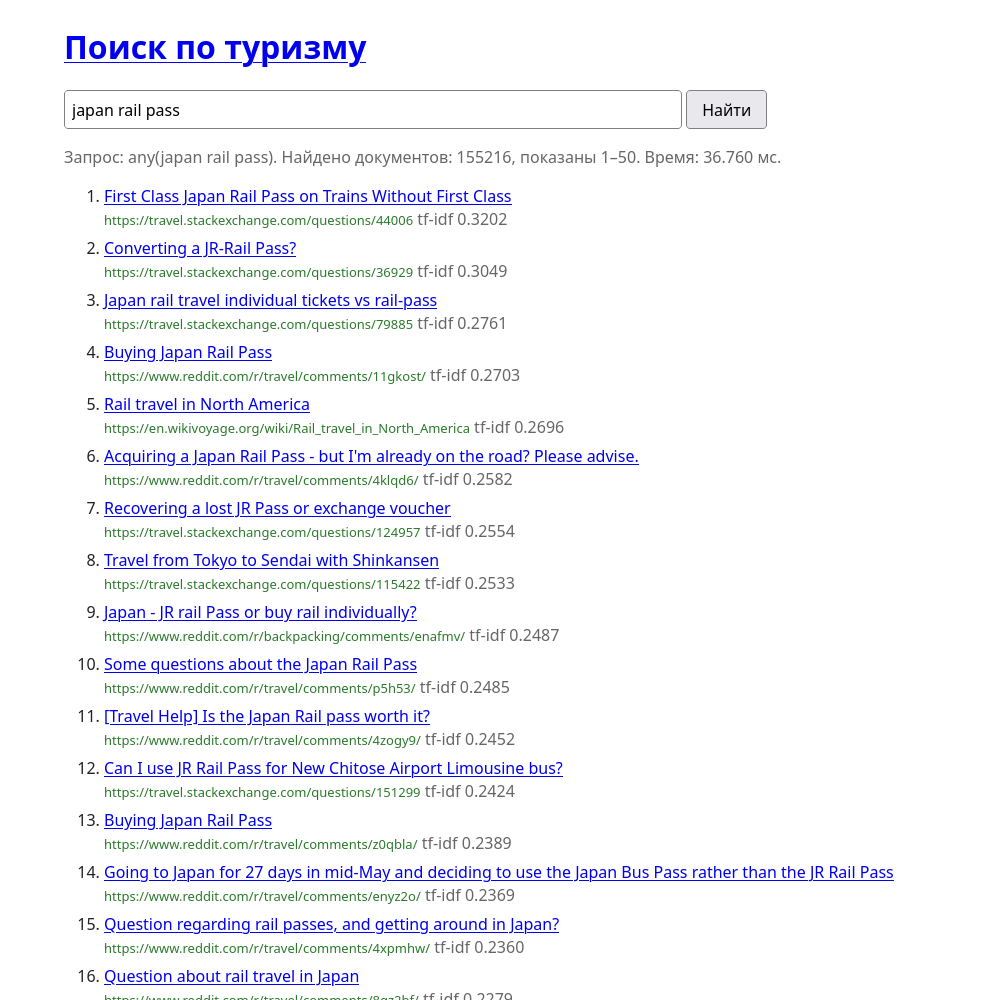
\includegraphics[width=0.75\textwidth]{img/search.png}

Выдача веб-сервиса по индексу с частотами: нечёткий запрос \texttt{japan rail pass}, под каждым результатом --- оценка TF-IDF
\end{center}

\subsection{Неудачные запросы и причины}
\begin{itemize}
    \item \texttt{moscow aviation institute}: статья Wikipedia \enquote{Moscow Aviation Institute} в корпусе есть, но в нечёткой выдаче она 153-я, в строгом И --- 25-я. Выше --- короткие документы: \enquote{Moscow (disambiguation)}, вопрос о транзитной визе в аэропорту Москвы, другие авиационные институты. Длинная статья о МАИ содержит слова запроса, но они --- малая часть её длинного вектора, и косинус маленький (0,10). Нечёткий режим ещё и допускает документы только со словом \texttt{moscow}.
    \item \texttt{snorkeling coral reefs thailand} --- единственный запрос, где ранжирование хуже порядка по docID (NDCG@10 0,30 против 0,45). Подробные путеводители Wikivoyage с разделами о снорклинге в Таиланде (\enquote{Diving in Thailand}, \enquote{Ko Lipe}, \enquote{Ko Lanta}) в ранжированной выдаче на 17-м, 21-м и 31-м местах --- длинные документы проигрывают коротким постам. Булев поиск выдаёт сначала Wikivoyage и случайно оказался лучше.
    \item \texttt{lviv old town}, нечёткий (0 релевантных): выше всех --- документы с редким словом \texttt{lviv} и без \texttt{old town}: река Полтва, город Щитно, вопросы о дороге во Львов. Статья \enquote{Old Town (Lviv)} появляется только в строгом И (3-е место).
    \item \texttt{japan rail pass}: энциклопедическая статья Wikipedia \enquote{Japan Rail Pass} --- только 241-я (нечёткий) и 149-я (строгое И): тоже длинная.
\end{itemize}
Как улучшить, не ухудшая остальные запросы: нормировку по длине сделать мягче (pivoted normalization --- длина документа учитывается относительно средней) или взять BM25, где насыщение tf и нормировка по длине настраиваются параметрами; учитывать совпадение в заголовке (зонный поиск --- отдельная ЛР: у \enquote{Moscow Aviation Institute}, \enquote{Old Town (Lviv)}, \enquote{Japan Rail Pass} весь запрос и есть заголовок); в нечётком режиме давать бонус документам со всеми словами запроса или с близко стоящими словами (координатный индекс).

\section{Выводы}
Сделан ранжированный поиск по схеме TF-IDF lnc.ltc (косинус векторов документа и запроса): запрос из одних слов --- нечёткий (документы хотя бы с одним словом), запрос с операторами --- строгий булев с порядком по TF-IDF. Для этого в индекс ЛР7 добавлены частоты термов и длины векторов документов (флаг 4, индекс 966~МиБ со сжатием), а в поиск ЛР8 --- накопление оценок по спискам и сортировка; утилита командной строки и веб-сервис показывают оценку. На 12 запросах с разметкой вслепую ранжирование подняло NDCG@10 с 0,16 до 0,73 (строгое И) и до 0,50 (нечёткий запрос), P@10 --- с 0,20 до 0,68 и 0,50.

Недостатки и как их исправить:
\begin{itemize}
    \item Косинусная нормировка опускает длинные документы, целиком посвящённые предмету запроса (МАИ, путеводители по Таиланду, статья о JR Pass), и поднимает короткие посты. Исправление --- pivoted normalization или BM25 и учёт заголовков (зонный поиск).
    \item Нечёткий режим без бонуса за полноту совпадения: документы с одним редким словом обгоняют документы со всеми словами. Можно умножать оценку на долю найденных слов запроса или учитывать близость слов.
    \item Ранжирование в 10--90 раз медленнее булева поиска: распаковываются полные списки всех слов, включая служебные, и сортируются все найденные документы. Ускорения: пропускать слова с малым idf или обрабатывать их последними с отсечением (MaxScore, WAND), выбирать первые $k$ результатов кучей вместо полной сортировки, в булевом режиме считать оценки только для найденных документов, держать длины векторов отдельным плотным массивом.
    \item Память индексации выросла до 4~ГиБ из-за частот --- хранить их в памяти компактнее (1--2 байта или сразу VByte).
    \item Оценка качества: 12 запросов и разметка одним оценщиком-моделью на запрос --- мало и субъективно; посты Reddit без комментариев не могут быть полностью релевантными, что занижает метрики систем, поднимающих посты.
\end{itemize}
